\section{Results}

\subsection{Imputation accuracy using 1M tagging SNPs}
The coverage for common variants (\gls{MAF} greater than 0.05) across all populations using 1M tagging variants is 0.93 (figure \ref{fig:f10}) suggesting that a 1M density array could potentially capture substantial proportions of variation across Africa. Using the hybrid approach improved the efficiency of tagging (figure \ref{fig:f10}) and using 10 cycles further improved the efficiency over using fewer cycles (data not shown).

\begin{figure}[htp]
\centering
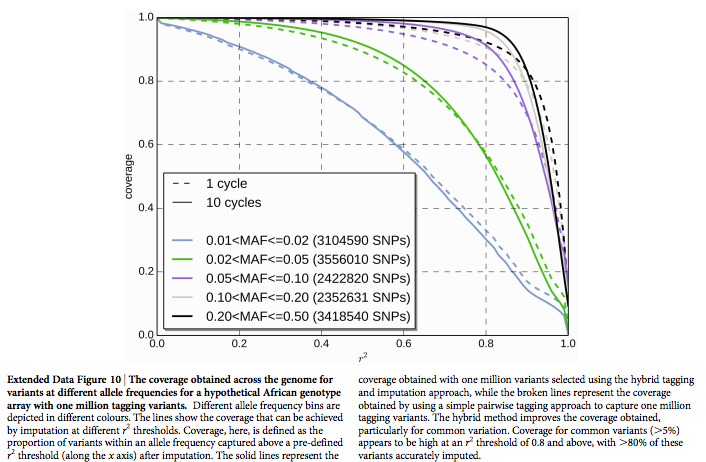
\includegraphics[trim={0 4cm 0cm 1cm},clip,width=0.8\textwidth]{fig/f10}
\caption[Imputation accuracy for a hypothetical 1M SNP array.]{
The coverage obtained across the genome for variants at different allele frequencies for a hypothetical African genotype array with one million tagging variants. Different allele frequency bins are depicted in different colours. The lines show the coverage that can be achieved by imputation at different \gls{r2} thresholds. Coverage, here, is defined as the proportion of variants within an allele frequency captured above a pre-defined \gls{r2} threshold (along the x axis) after imputation. The solid lines represent the coverage obtained with one million variants selected using the hybrid tagging and imputation approach, while the broken lines represent the coverage obtained by using a simple pairwise tagging approach to capture one million tagging variants. The hybrid method improves the coverage obtained, particularly for common variation. Coverage for common variants (\gls{MAF} greater than 0.05) appears to be high at an \gls{r2} threshold of 0.8 and above, with 80\% of these variants accurately imputed.
}
\label{fig:f10}
\end{figure}

\subsection{Comparison of RagTagger with existing methods}
RagTagger uses less than 1GB of memory when selecting tag SNPs from a 2\gls{Mbp} fragment and runs to completion in a few minutes. TAGster\cite{Xu2007} uses more than 10GB of memory (16.5GB) on the same 2\gls{Mbp} fragment and takes longer than a day to run to completion (1.18 days). TAGster fails to run to completion when run across the whole genome and RagTagger finishes in 3 hours using less than 10GB of memory. FESTA (Fragmented Exhaustive Search for TAgSNPs)\cite{Qin15012006} failed to run to completion within 48 hours.